\documentclass{scrbook}
% !TEX ROOT = main.tex

\usepackage{afterpage}
\usepackage{amsmath}
\usepackage[ngerman]{babel}
\usepackage{blindtext}
\usepackage{csquotes}
% \usepackage{enumitem} % error: underfull hbox
\usepackage{eurosym}
\usepackage{fancyhdr}
\usepackage{float}
\usepackage{fontawesome}
\usepackage[T1]{fontenc}
\usepackage{geometry}
\usepackage[pdftex]{graphicx}
%\usepackage[scaled=0.81]{helvet}     % Schriftart fuer Resos
\usepackage{hyperref}
\usepackage[utf8]{inputenc}
\usepackage{libertine}
\usepackage{lmodern}     % Ersatz fuer Computer Modern-Schriften
\usepackage{mdwlist}     % Änderung der Zeilenabstände bei itemize und enumerate
\usepackage{microtype}
\usepackage{minitoc}
\usepackage{outlines}
\usepackage{paralist}
\usepackage{pdfpages}
\usepackage{subcaption}
\usepackage{tcolorbox}
\usepackage{titlesec}
\usepackage{tocloft}
\usepackage{todonotes}
\usepackage{ulem}
\usepackage{url}
\usepackage{wrapfig}
\usepackage{xcolor}
\usepackage{xpatch}
% \usepackage[draft, markup=underlined]{changes}

  % braucht man das?
%\usepackage{titlesec}    % Abstand nach Überschriften neu definieren
%\titlespacing{\subsection}{0ex}{3ex}{-1ex}
%\titlespacing{\subsubsection}{0ex}{3ex}{-1ex}

\definecolor{urlred}{HTML}{660000}
\hypersetup{ % Design der Hyperrefs
    colorlinks=true,
    linkcolor=black,    % Farbe der internen Links (u.a. Table of Contents)
    urlcolor=black,    % Farbe der url-links
    citecolor=black} % Farbe der Literaturverzeichnis-Links

\parindent 0pt                 % Absatzeinrücken verhindern (pck:blindtext)
\parskip 2pt                 % Absätze durch Lücke trennen

% Inhaltsverzeichnis
\renewcommand\cftbeforetoctitleskip{-1cm}

% Suche nach Grafiken in ./media und .:
% \graphicspath{{./media/}{./}}

% Satzspiegel
\geometry{papersize={154mm,216mm}, layout=a5paper, layouthoffset=3mm, layoutvoffset=3mm, inner=20mm, outer=15mm, top=15mm, bottom=15mm, heightrounded, marginparwidth=7mm, marginparsep=5mm}
\setlength{\parindent}{0pt}

% Schriftarten
\fontfamily{pag}\selectfont % Avantgar
%\renewcommand{\sfdefault}{phv}
% \newenvironment{resofont}{\fontfamily{phv}\selectfont}{\par}

% itemize item titlespacing
% ??? ohne enumitem

% Headlines
\pagestyle{fancy}
\fancyhf{}
\definecolor{unicolor}{HTML}{B5152B}
\renewcommand{\headrulewidth}{1.5pt} % Strich unterm Header
\renewcommand{\footrulewidth}{0pt} % Strich überm Footer
\renewcommand{\chaptermark}[1]{ \markboth{\quad \quad \quad \bfseries#1 \quad \quad}{}} % chapter Titel mit "Formatierung"
\renewcommand{\sectionmark}[1]{ \markright{#1 \quad \quad \quad}{}} % section Titel mit "Formatierung"
\newlength\FHoffset
\setlength\FHoffset{1cm}
\setlength{\headheight}{22pt}
\setlength{\headsep}{5mm}
\addtolength\headwidth{2\FHoffset} % andere Länge für Header als Text
\fancyheadoffset{\FHoffset}
\fancyfootoffset{\FHoffset}

\renewcommand{\headrule}{\hbox to\headwidth{%
  \color{unicolor}\leaders\hrule height \headrulewidth\hfill}}
% \xpretocmd\headrule{\color{unicolor}}{}{\PatchFailed}

\fancyhead[RO]{\large \rightmark}
\fancyhead[LE]{\large \leftmark}
\chead{}
% \rhead{\large \rightmark}

\fancyfoot[OR]{
  \begin{tikzpicture}
    \node at (0.5, 0) {
\includegraphics[width=1cm, height=1cm]{vorlagen/logo2.png}};
    \draw [thick, unicolor] (0,-0.5) -- (0,0.5);
    \node at (-0.5,0) {\Large \thepage};
  \end{tikzpicture}
}

\fancyfoot[EL]{
  \begin{tikzpicture}
    \node at (-0.5, 0) {
\includegraphics[width=1cm, height=1cm]{vorlagen/logo2.png}};
    \draw [thick, unicolor] (0,-0.5) -- (0,0.5);
    \node at (0.5,0) {\Large \thepage};
  \end{tikzpicture}
}

% Boxen etwa für Abstimmungen in Plenen
\newenvironment{success}[1]{
  \begin{center}
    \begin{tcolorbox}[colback=green!5!white,colframe=green!60!black, title=#1]
    }
    {
    \end{tcolorbox}
  \end{center}
}

\newenvironment{info}[1]{
  \begin{center}
    \begin{tcolorbox}[colback=blue!5!white,colframe=blue!60!black, title=#1]
    }
    {
    \end{tcolorbox}
  \end{center}
}

\newenvironment{danger}[1]{
  \begin{center}
    \begin{tcolorbox}[colback=yellow!5!white,colframe=yellow!75!black, title=#1]
    }
    {
    \end{tcolorbox}
  \end{center}
}

% Chapter Formatting
\newcommand{\tocchapter}{
  \titlespacing*{\chapter}{0pt}{-5pt}{40pt}
  \titleformat{\chapter}[display]
    {\normalfont\bfseries\scshape\filcenter}
    {\Huge\thechapter}
    {1ex}
    {\color{unicolor}\titlerule[7pt]
    \vspace{4ex}%
    \color{black}
    \Huge}
    [\vspace{1ex}%
    \color{unicolor}
    {\titlerule[7pt]}
    \setlength{\mtcindent}{5pt}
    \minitoc
    \vspace{2cm}
    {
\includegraphics[scale=0.2]{vorlagen/logo.png}}
    {\newpage}]

    \assignpagestyle{\chapter}{empty}
}


\newcommand{\emptychapter}{
  \titleformat{\chapter}[display]
    {\normalfont\bfseries\scshape\filcenter}
    {\Huge\thechapter}
    {1ex}
    {\color{unicolor}\titlerule[7pt]
    \vspace{4ex}%
    \color{black}
    \Huge}
    [\vspace{1ex}%
    \color{unicolor}
    {\titlerule[7pt]}
    \vspace{7cm}
    {
\includegraphics[scale=0.4]{vorlagen/logo.png}}
    {\newpage}]

    \assignpagestyle{\chapter}{empty}
}

% used for resos and pospaps
% \pagestyle{empty}
% \cfoot{}
% \lfoot{Zusammenkunft aller Physik-Fachschaften}
% \rfoot{www.zapfev.de\\stapf@zapf.in}
% \renewcommand{\headrulewidth}{0pt}
% \renewcommand{\footrulewidth}{0.1pt}
% \newcommand{\gen}{*innen}

%Unterdrückt Section und Subsection Nummern, also werden nur Chapter Nummer angezeigt
\setcounter{secnumdepth}{0}


%zusätzliche Packages nur für den Mantelbogen
\usepackage[absolute]{textpos}  % Zum Positionieren der Grafiken
\usepackage{rotating}           % Zum Drehen von Text
\setlength{\parindent}{0pt}
\usepackage{background}
\backgroundsetup{
scale=1.1,
angle=0,
opacity=1,  %% adjust
contents={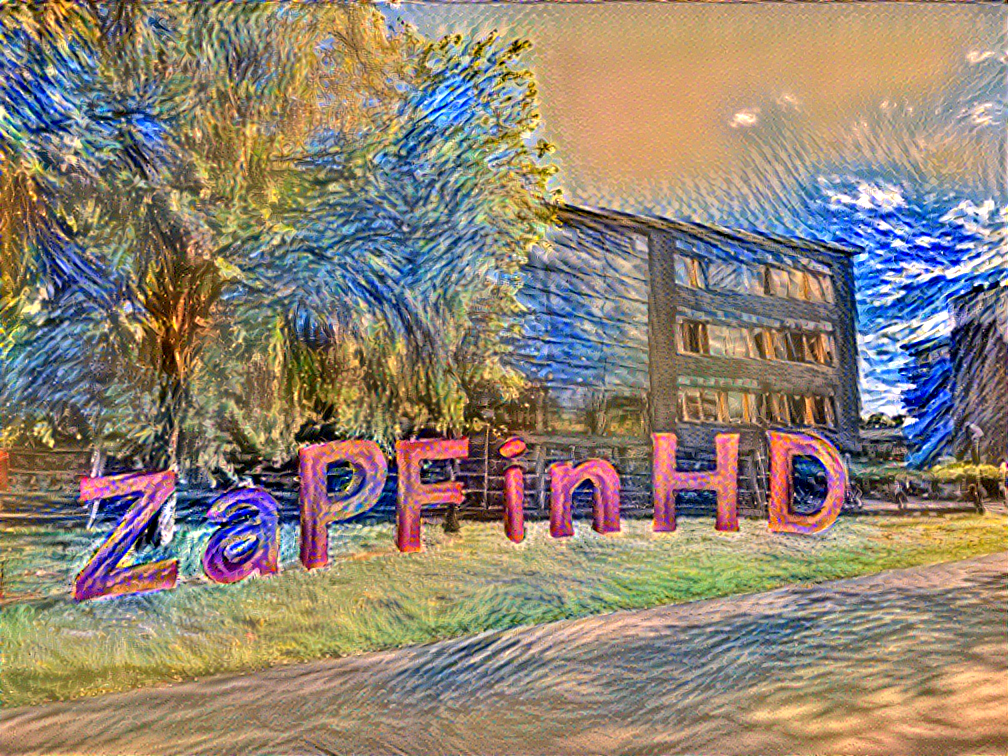
\includegraphics[width=\paperwidth]{vorlagen/vangogh}}
}
\usepackage{geometry}
\geometry{bottom=10mm}

\begin{document}

% VORDERSEITE, AUSSEN %
\pagestyle{empty}
\centering
\vspace*{-10mm}


\includegraphics[width=60mm]{vorlagen/logo_breit} 

\vspace*{14cm} \centering \fontsize{40}{48} \textbf{Tagungsreader}
\normalsize

%\begin{textblock*}{148mm}[0,0](0mm,100mm)
    %
\includegraphics[width=148mm]{logo_breit} 
%\end{textblock*}
      
% TeX denkt, dass die Seite noch leer ist und macht deswegen keinen
% pagebreak. Das \null täuscht TeX und alle sind glücklich (bis auf die
% Perfektionisten natürlich)
\null
\newpage
\backgroundsetup{
scale=1.1,
angle=0,
opacity=1,  %% adjust
contents={}
}
% VORDERSEITE, INNEN %
\vspace*{\fill}
    \begin{tabular*}{\textwidth}{ll}
        \multicolumn{2}{l}{
            \parbox{\textwidth}{
                Der Redaktionsschluss für diesen Text war am 21. November 2018. Wir freuen uns
                sehr über Komplimente, Blumen und Kuchen -- melde dich bei
                \href{mailto:akzapf@mathphys.stura.uni-heidelberg.de}{akzapf@mathphys.stura.uni-heidelberg.de}. \\
                Vielen Dank an dieser Stelle noch mal für keine Hilfe ... 
            }
            \vspace{1cm}
        }\\
	\multicolumn{2}{l}{
	\parbox{0.77\textwidth}{
       	\textbf{Bild Copyrights}
       	\begin{tabbing}
        Christoph Blattgerste \quad \quad \= Editor \\
		Christoph Blattgerste \quad \quad \=  Titelbild (Cover) \\		
		Henrik Reinstädtler\> Titelbild van Gogh Stil \\
		Lennart Stipulkowski \> ZaPF Logo \\
		Christoph Blattgerste\footnotemark \> Skizze \\
        Christoph Blattgerste \quad \quad \= Design	
		\end{tabbing}
       	}
      }\\  

        \textbf{Impressum} \\ \\
        Herausgeber & Studienfachschaft Physik, Universität Heidelberg \\
        & Im Neuenheimer Feld 205, Raum 01.301\\
        & 69120 Heidelberg\\
        V.\,i.\,S.\,d.\,P. & Christoph Blattgerste\\
        & Im Neuenheimer Feld 205, Raum 01.301\\
        & 69120 Heidelberg\\
    \end{tabular*}

        \footnotetext[1]{www.xkcd.com}
        \footnotetext[2]{www.samuelscherer.de}                
    \vfill


\null
\newpage

% RÜCKSEITE, INNEN %
% wird nicht verwendet -> stattdessen Schlussworte
\pagestyle{empty}
% Campusplan
\null
\backgroundsetup{
scale=1.02,
angle=90,
opacity=1,  %% adjust
contents={
\includegraphics[angle=90, width=5cm]{vorlagen/exzellente}}
}

\newpage

% RÜCKSEITE, AUSSEN %
\pagestyle{empty}
\null
\backgroundsetup{
scale=1.075,
angle=270,
opacity=1,  %% adjust
contents={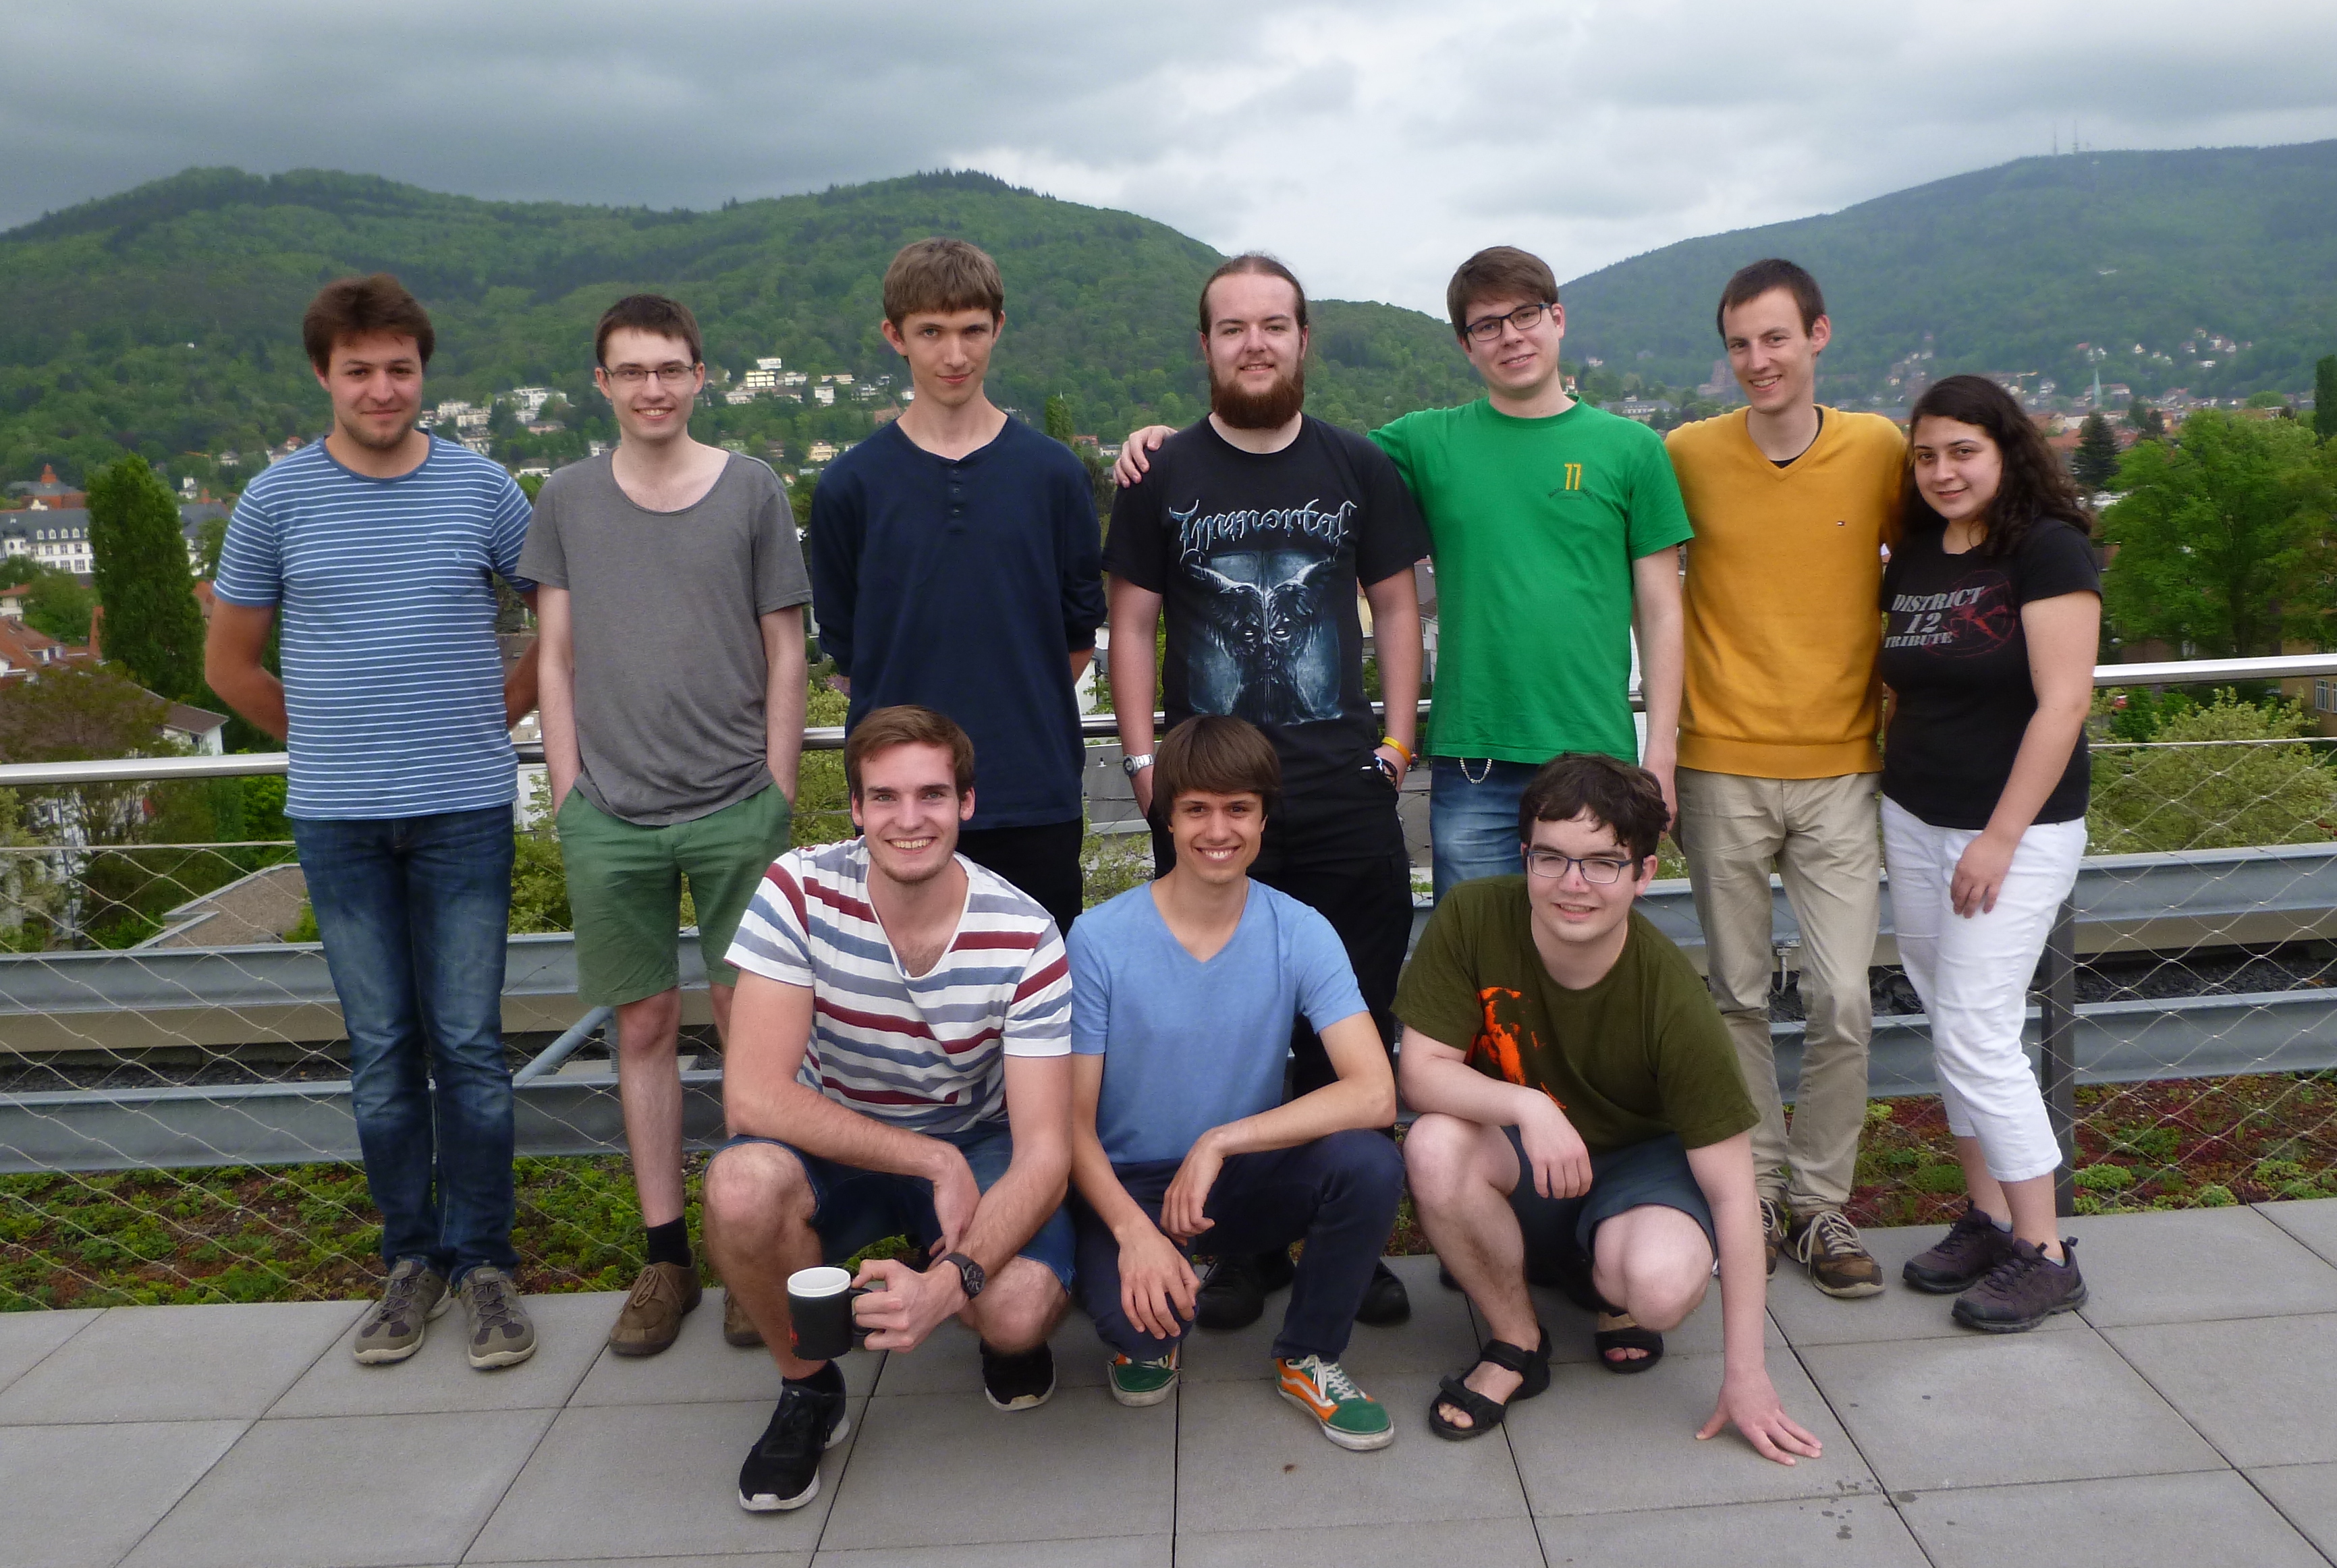
\includegraphics[angle=90, width=10cm]{bilder/orga.png}}
}

\Huge \textbf{Mit fachschaftlichen Grüßen}

\vspace{15cm}

\Huge \textbf{Deine Orga}
%\begin{textblock}{30}(8.8,1)
%\includegraphics[width=50mm]{MathPhysInfoLogo} 
%\end{textblock}
\newpage
\end{document}
